\documentclass{etit-workshop-protokoll}

%\kursnummer{0}
%\kurstitel{Leitfaden und Vorlage zur Ausarbeitung}

%\kursnummer{1}
%\kurstitel{Messwerterfassung und regenerative Energieerzeugung}

\kursnummer{2}
\kurstitel{Analoge Filter und Schaltungsanalyse}

%\kursnummer{3}
%\kurstitel{Sensorik}

%\kursnummer{4}
%\kurstitel{Digitale Signalverarbeitung}


\gruppennummer{51}


\teilnehmer{Lukas}{Ringle}{2258752}{uutpe}{uutpe@student.kit.edu}
\teilnehmer{Henning}{Heeb}{2294399}{uckgt}{uckgt@student.kit.edu}
\teilnehmer{Fabian}{Moritz}{2314434}{ufjkg}{ufjkg@student.kit.edu}

\usepackage{graphicx}
\usepackage{siunitx}

\begin{document}

\maketitle

\pagestyle{empty}% % leere Kopfzeile
\begin{abstract}
\section*{Zielsetzung}
Aufgabe der Arbeit ist die Entwicklung eines 2-Band-Equalizers. Dieser soll durch unabhängig Hoch- und Tiefpassfilter realisiert werden, deren Ausgänge danach in einer Addiererschaltung zusammengeführt werden. Diese Art des Zusammenführens ermöglicht eine genauere Soundeinstellung.

\end{abstract}
\clearpage % neue Seite beginnen
\pagestyle{scrheadings} % Kopfzeilen zuruecksetzen

\tableofcontents
\listoffigures
\listoftables
\clearpage % neue Seite beginnen

\section{Aufgabenverteilung}

Die Aufgaben wurden gemeinsam bearbeitet. Lukas hat einen großen Beitrag zur Arbeit durch seinen intensive Recherche zum Thema Filter geleistet. Die Simulation in LT Spice und die Dimensionierung der Schaltungen wurde geimeinschaftlich erledigt. Henning und Lukas bauten zusammen die physische Schaltung auf und Fabian kümmerte sich um die Organisation der LateX Dokumentaion, an der selbstverständlich alle Gruppenmitglieder mitwirkten.
\section{Grundlagen}

\section{Filterschaltung}
In diesem Kapitel werden die Filterschaltungen zum splitten des Frequenzbereiches des Eingangssignals geplant, simuliert und gebaut.

\subsection{Methoden}
Das Teilen des Eingangssignals in zwei Frequenzbereiche lässt sich mit einem Hoch- und einem Tiefpass realisieren. Wichtig ist hierbei, dass beide Filter die Gleiche Grenzfrequenz besitzen, damit keine Frequenzen 'verloren gehen'. 1kHz ist eine sinnvolle Grenzfrequenz, da diese Frequenz in der logarithmischen Mitte zwischen 200Hz und 5000Hz liegt. Diese Werte entsprechen dem Frequenzintervall des Hauptsprachbereichs welche sich dem Diagramm\cite{Hoerbereichdiagramm} der Aufgabenstellung entnehmen lassen. \\
Des weiteren müssen beide Filter das Eingangssignal um den Faktor 1 verstärken und von 2ter Ordnung sein. Dies lässt sich mit, nach ihren Erfindern benannten, Sallen-Key Filtern erreichen.
Diese Annahme bezogen wir aus dem LEN-Skript.\\
Um eine Verstärkung von 1 zu erzielen bedarf es einer direkten Rückkopplung des Ausgangssignals auf den invertierenden Eingang des OpAmps. Die Schaltung im Computerprogramm LTSpice gebaut ist in folgender Abbildung zu sehen:
\begin{figure}[H]
	\centering
	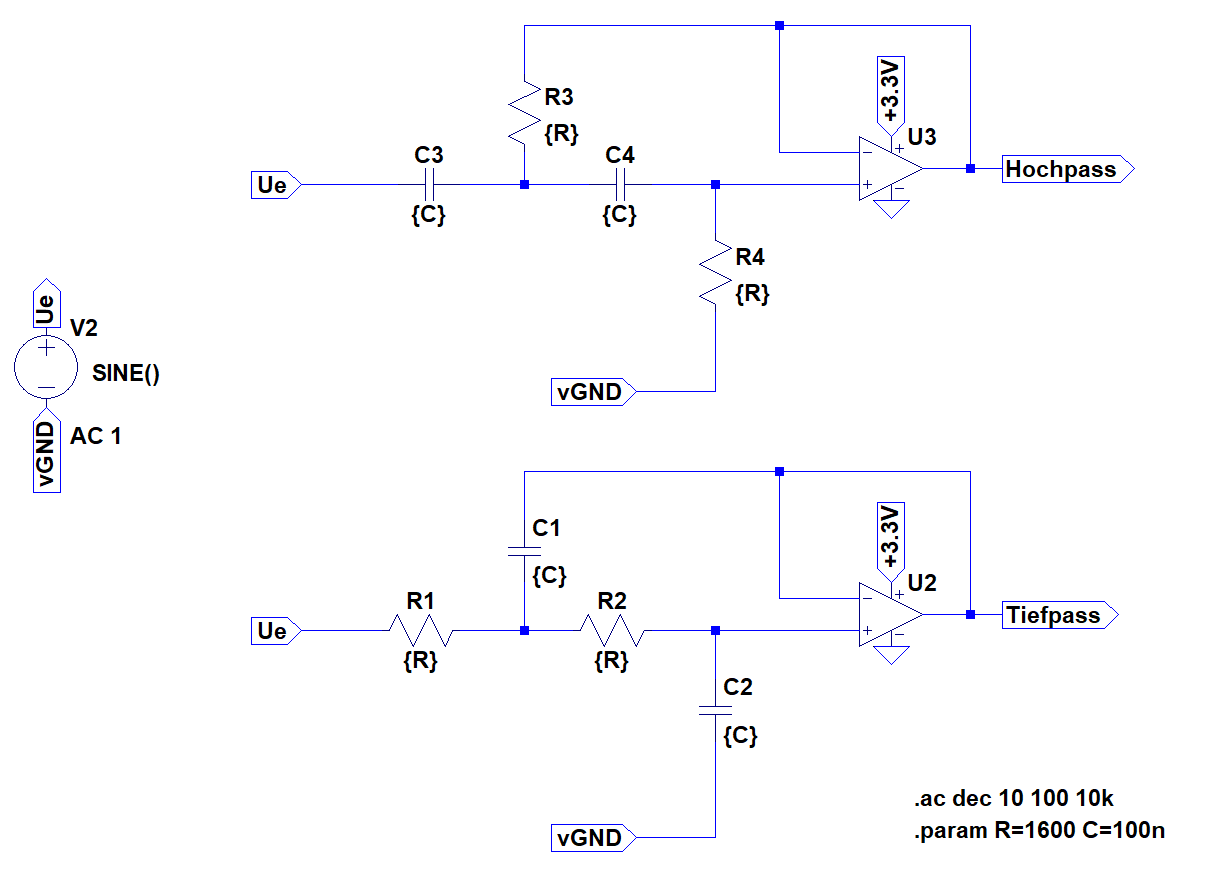
\includegraphics[width=1\textwidth]{pics/SpiceSchaltungFilter.PNG}
	\caption{Aufbau Hoch- und Tiefpass in LTSpice}
\end{figure}
Im folgenden werden die Werte für die Widerstände und die Kondensatoren bestimmt.
Für die Güte des Tiefpass-Filter gilt:
$$ Q = \frac{1}{2}\cdot\sqrt{\frac{C_{1}}{C_{2}}} $$

Die Anforderungen an die Filter verlangen eine Güte von 0,5. Daher gilt $C_{1}=C_{2}$.\\
Für $\omega_{0}$ beim Tiefpass ist gegeben:
$$\omega_{0}=\frac{1}{R\cdot\sqrt{C_{1} \cdot C_{2}}}$$

Da $C_{1}$ und $C_{2}$ den gleichen Wert haben sollen und die Grenzfrequenz $f_{0}=1\si{\kilo\hertz}$ betragen soll, ergibt sich:
$$\omega_{0}=2\pi f_{0} \approx 6283\si{\hertz} \, \Leftrightarrow \,\omega_{0}=\frac{1}{R\cdot C}\approx 6283\si{\hertz} $$

Da die uns zur Verfügung stehende Anzahl and verschiedenen Widerständen größer ist als die der Kondensatoren, haben wir $C_{1}=C_{2}=100\si{\nano\farad}$ gewählt.

Daraus ergibt sich $R=1592\si{\ohm}$. Damit erfüllt der Tiefpass-Filter alle geforderten Eigenschaften. \\
Für die Güte des Hochpass-Filter gilt:
$$Q=\frac{1}{2}\cdot\sqrt{\frac{R_{1}}{R_{2}}}$$

Es muss $R_{1}=R_{2}$ gewählt werden um auch beim Hochpass eine Güte von 0,5 zu bekommen.
Für $\omega_{0}$ ist gegeben:
$$\omega_{0} = \frac{1}{C\cdot\sqrt{R_{1}\cdot R_{2}}}$$

Aus $R_{1}=R_{2}$ folgt:
$$\omega_{0} = \frac{1}{C\cdot R}=6283\si{\hertz}$$

Wir erhalten also die selbe Gleichung für die Eigenfrequenz wie beim vorher besprochenen Tiefpass-Filter. Wenn in beiden Filtern jeweils alle Kondensatoren und alle Widerstände den gleichen Wert haben, bekommen wir bei beiden Filtern die selbe Grenzfrequenz. Selbstverständlich ist möglich beim Tiefpass-Filter andere Werte zu nehmen als beim Hochpass-Filter. So lange man jedoch $C_{1}=C_{2}$ und $R_{1}=R_{2}$ gilt, weisen die Filter immer exakt das selbe Verhalten auf.\\
Wie schon erwähnt entscheiden wir uns für $C=100\si{\nano\farad}$, auf Grund der uns zur Verfügung stehenden Kondensatoren. Da sich ein exaktes $R=6283\si{\ohm}$ mit unseren Möglichkeiten nicht realisieren lässt, bauen wir die Filter mit einem 1500\si{\ohm} und einem 100\si{\ohm} Widerstand in Reihe geschaltet und erhalten so $R=1600\si{\ohm}$.\\
Somit gilt für unsere Grenzfrequenz:
$$\omega_{0}=\frac{1}{1600\si{\ohm}\cdot 100\si{\nano\farad}}=6250\si{\hertz}\Rightarrow f_{0}=\frac{\omega_{0}}{2\pi}\approx 995\si{\hertz}$$

Diese kleinen Abweichung von unseren angedachten 1\si{\kilo\hertz} macht nichts weiter aus, da wir trotzdem bei beiden Filtern die selbe Grenzfrequenz erhalten.
Somit entspricht die Schaltung allen Anforderungen der Aufgabenstellung.\\
Die Übertragungsfunktion des Tiefpasses lässt sich mittels der Knotengleichungen bestimmen:
\begin{align*}
K1:\qquad &\frac{U_{e}-U_{1}}{R}-\frac{U_{1}-U_{a}}{Z_{C}}-\frac{U_{1}-U_{2}}{R}=0\\
K2:\qquad &\frac{U_{1}-U_{2}}{R}-\frac{U_{2}}{Z_{C}}=0
\end{align*}
Da wir einen Verstärkungsfaktor von 1 haben, ergibt sich nach der Spannungsteiler-Regel:
$$U_{a}=1\cdot U_{2}$$
Nach einigem Umformen und Einsetzen von $Z_{C}=\frac{1}{j\omega C}$ erhält man die Übertragungsfunktion des Tiefpass-Filters:
\begin{align*}
\frac{U_{a}}{U_{e}}&=\,\frac{Z_{C}^2}{Z_{C}^2+2R Z_{C}+R^2}\,=\,\frac{-\frac{1}{\omega^2 C^2}}{\frac{2R}{j\omega C}-\frac{1}{\omega^2 C^2}+R^2}\\
&=\, \frac{1}{2j\omega RC+1-\omega^2 R^2C^2}
\end{align*}
Analog lässt sich beim Hochpass vorgehen:
\begin{align*}
K1:\qquad &\frac{U_{e}-U_{1}}{Z_{C}}-\frac{U_{1}-U_{a}}{R}-\frac{U_{1}-U_{2}}{Z_{C}}=0\\
K2:\qquad &\frac{U_{1}-U_{2}}{Z_{C}}-\frac{U_{2}}{R}=0
\end{align*}
Wieder gilt die Spannungsteiler-Regel mit $U_{a}=U_{2}$.
Auch hier gehen wir analog zum Tiefpass vor um die Übertragungsfunktion zu erhalten:
\begin{align*}
\frac{U_{a}}{U_{e}}&=\,\frac{R^2}{2Z_{C}R+R^2+Z_{C}^2}\,=\,\frac{R^2}{\frac{2R}{j\omega C}+R^2-\frac{1}{\omega^2 C^2}}\\
&=\, \frac{-\omega^2 R^2 C^2}{2R\omega C-\omega^2 R^2 C^2+1}
\end{align*} 
Die von uns gebauten Filter-Schaltungen auf dem Steckbrett sind in folgenden Abbildungen zu sehen:

\begin{figure}[H]
	\subfigure[Hochpass]{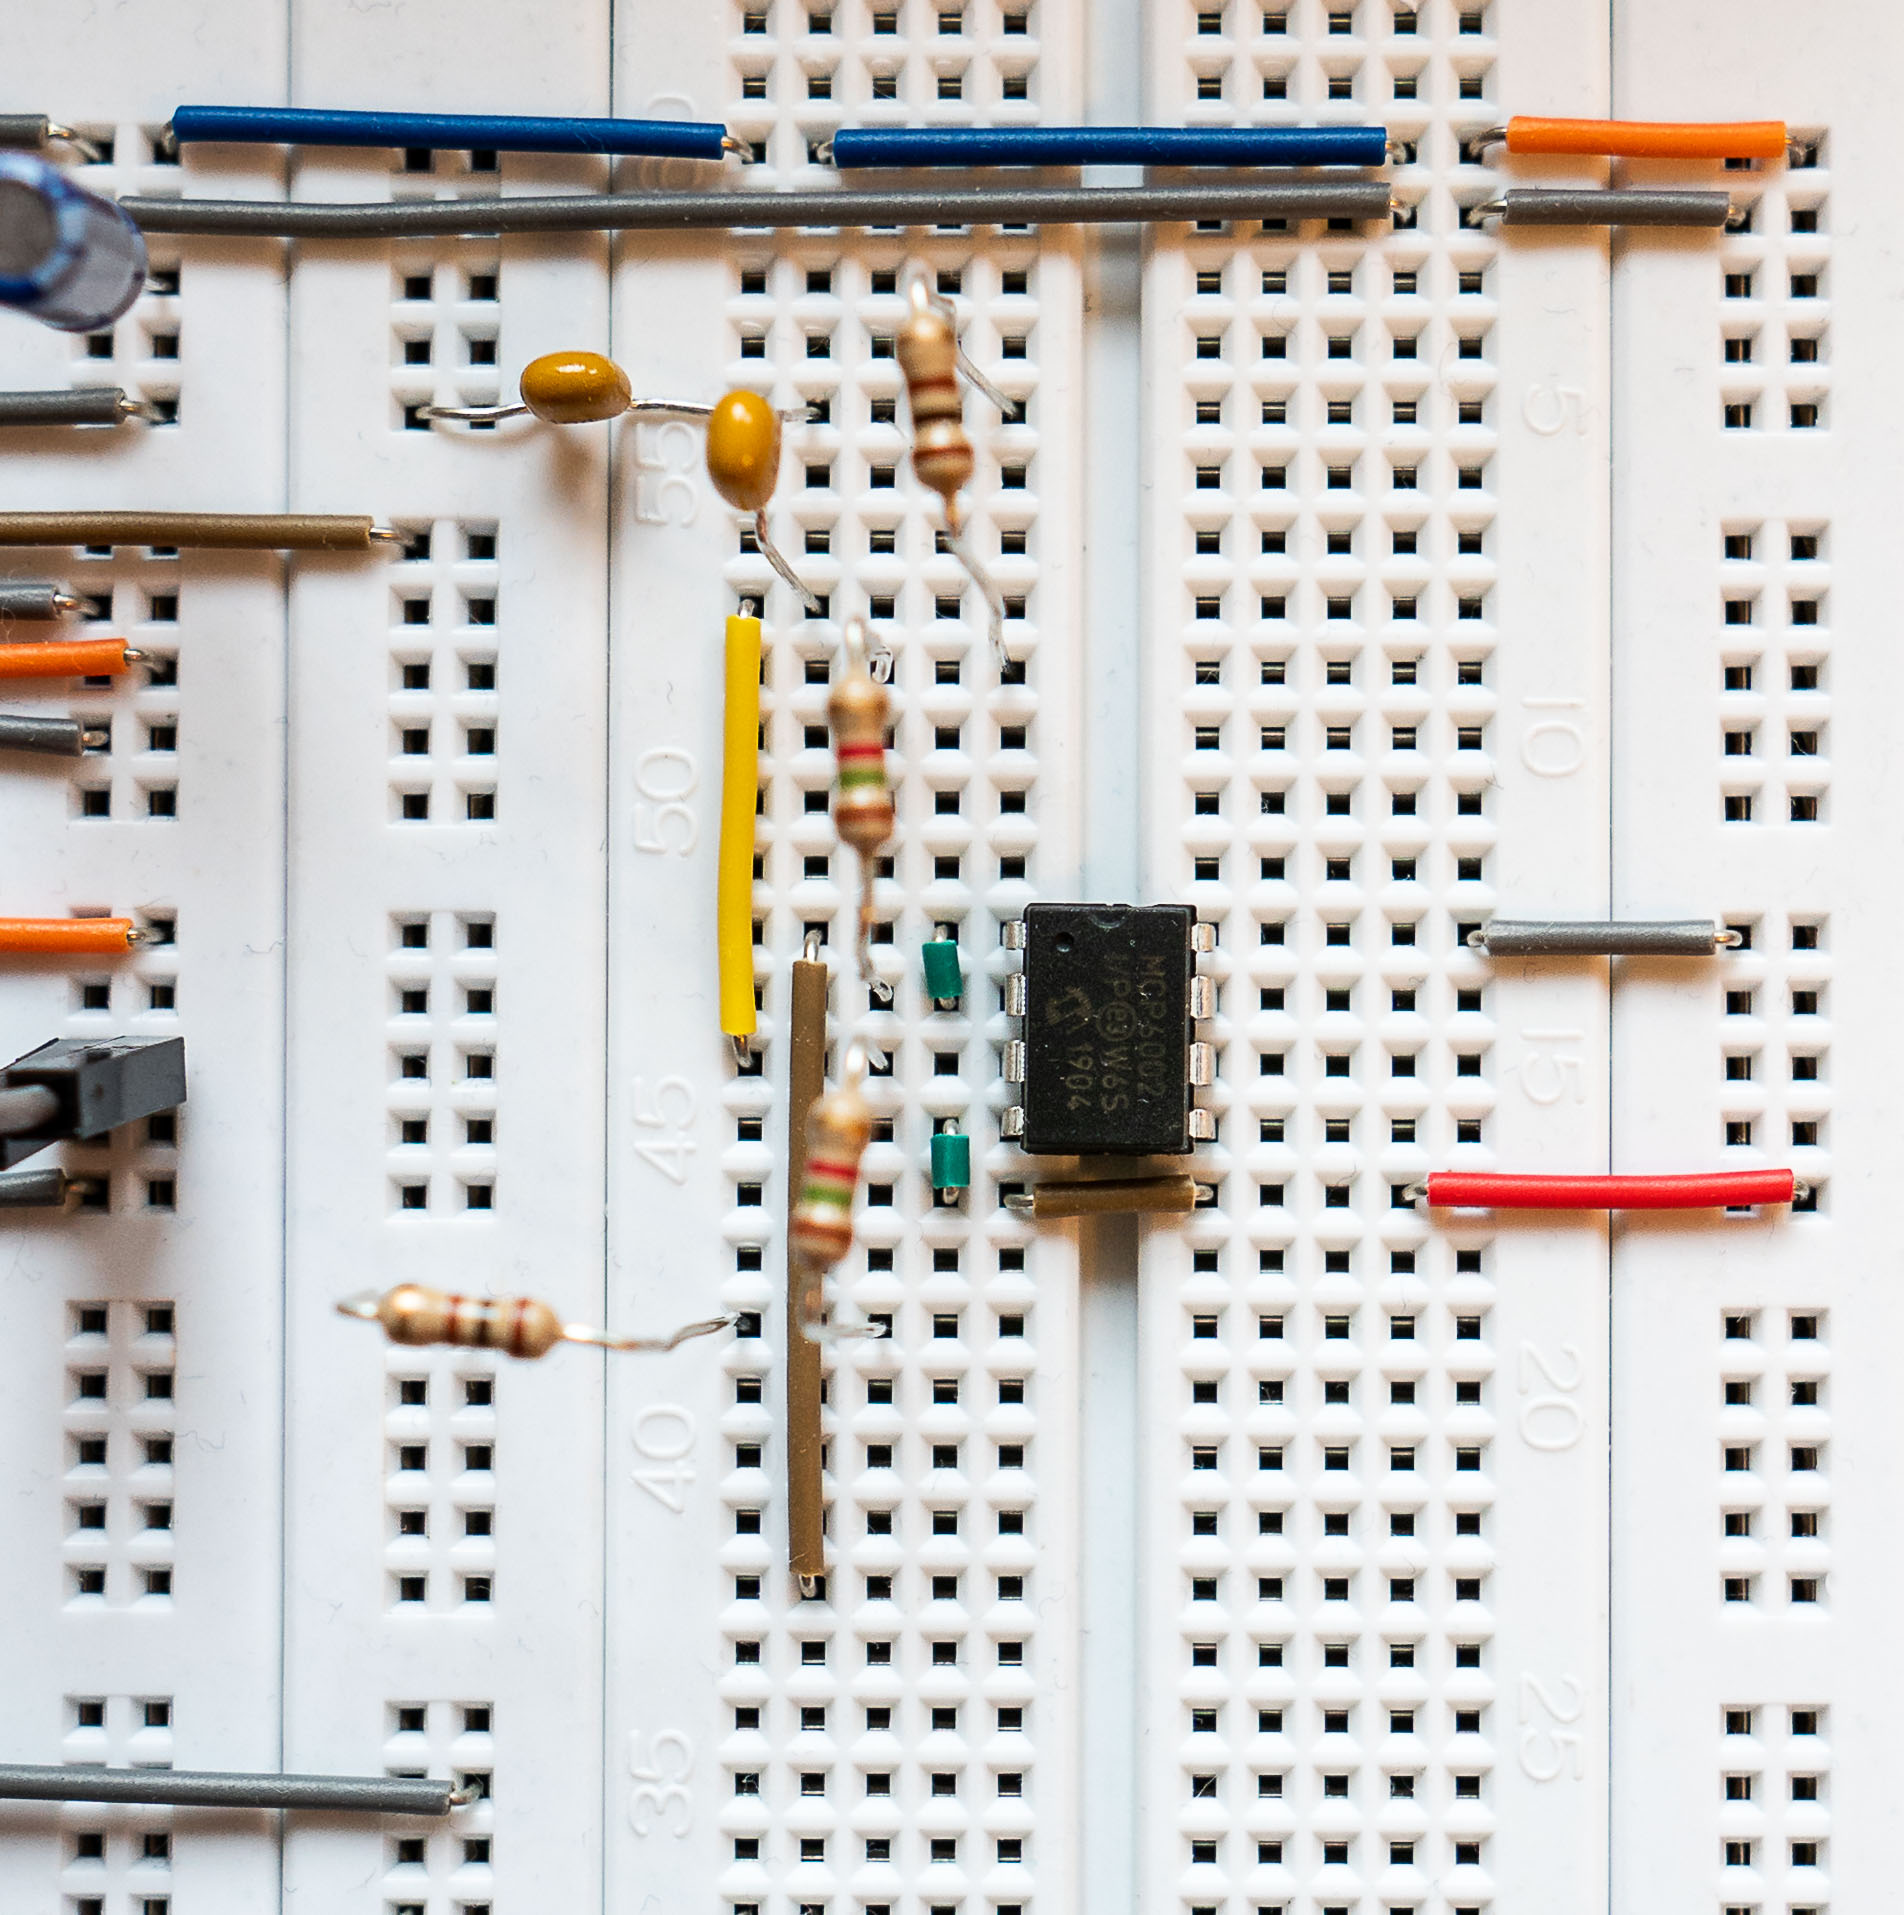
\includegraphics[width=0.45\textwidth]{pics/Hochpass aufgebaut.jpg}}
	\quad
  	\subfigure[Tiefpass]{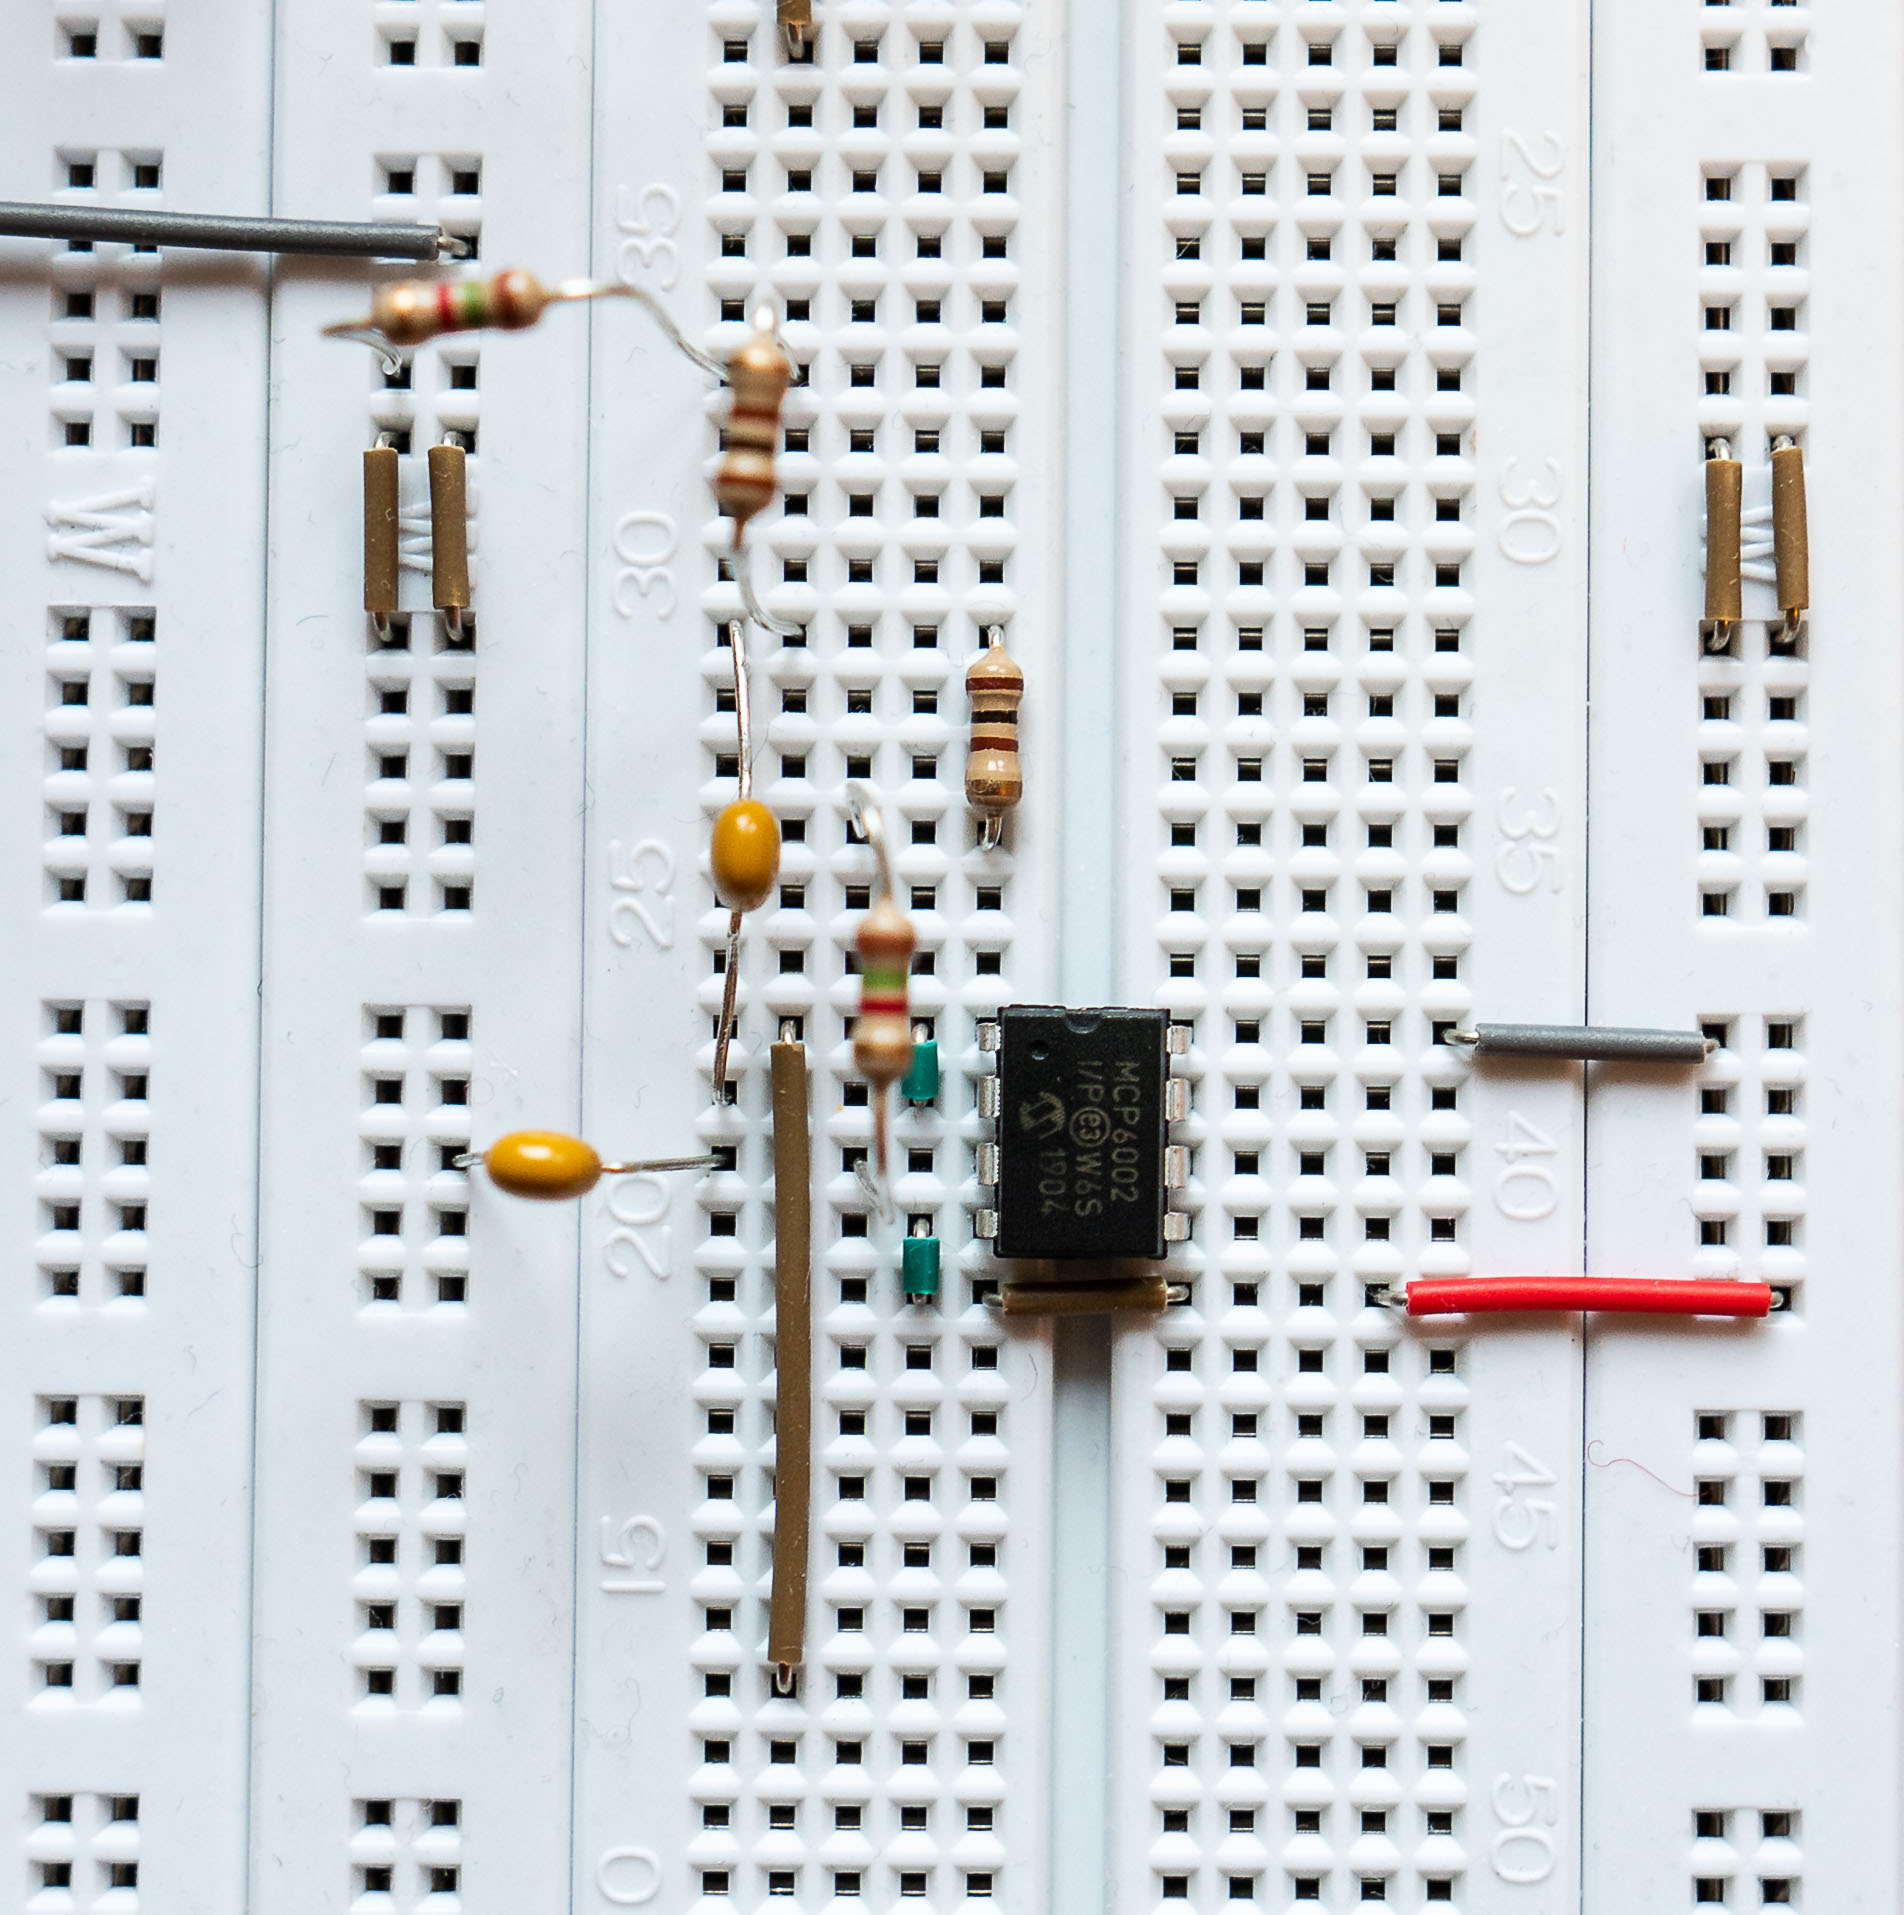
\includegraphics[width=0.45\textwidth]{pics/Tiefpass aufgebaut.jpg}}
  	\caption{Aufbau Hoch- und Tiefpass}  	
  	\label{Aufbau Hoch- und Tiefpass}
\end{figure}
\newpage
\subsection{Ergebnisse}
Um die korrekte Funktionsweise unserer auf dem Steckbrett gebauten Filterschaltungen nachzuweisen, wird ein sinusförmiges Eingangssignal verschiedener Frequenzen auf die Schaltungsteile gegeben. Vergleicht man das vom TI-Board erzeugte Signal mit dem Ausgangssignal des jeweiligen Passes, lässt sich dessen Funktionsweise analysieren.\\
\begin{figure}[H]
	\centering
	\subfigure[Hochpass bei tiefen Frequenzen]{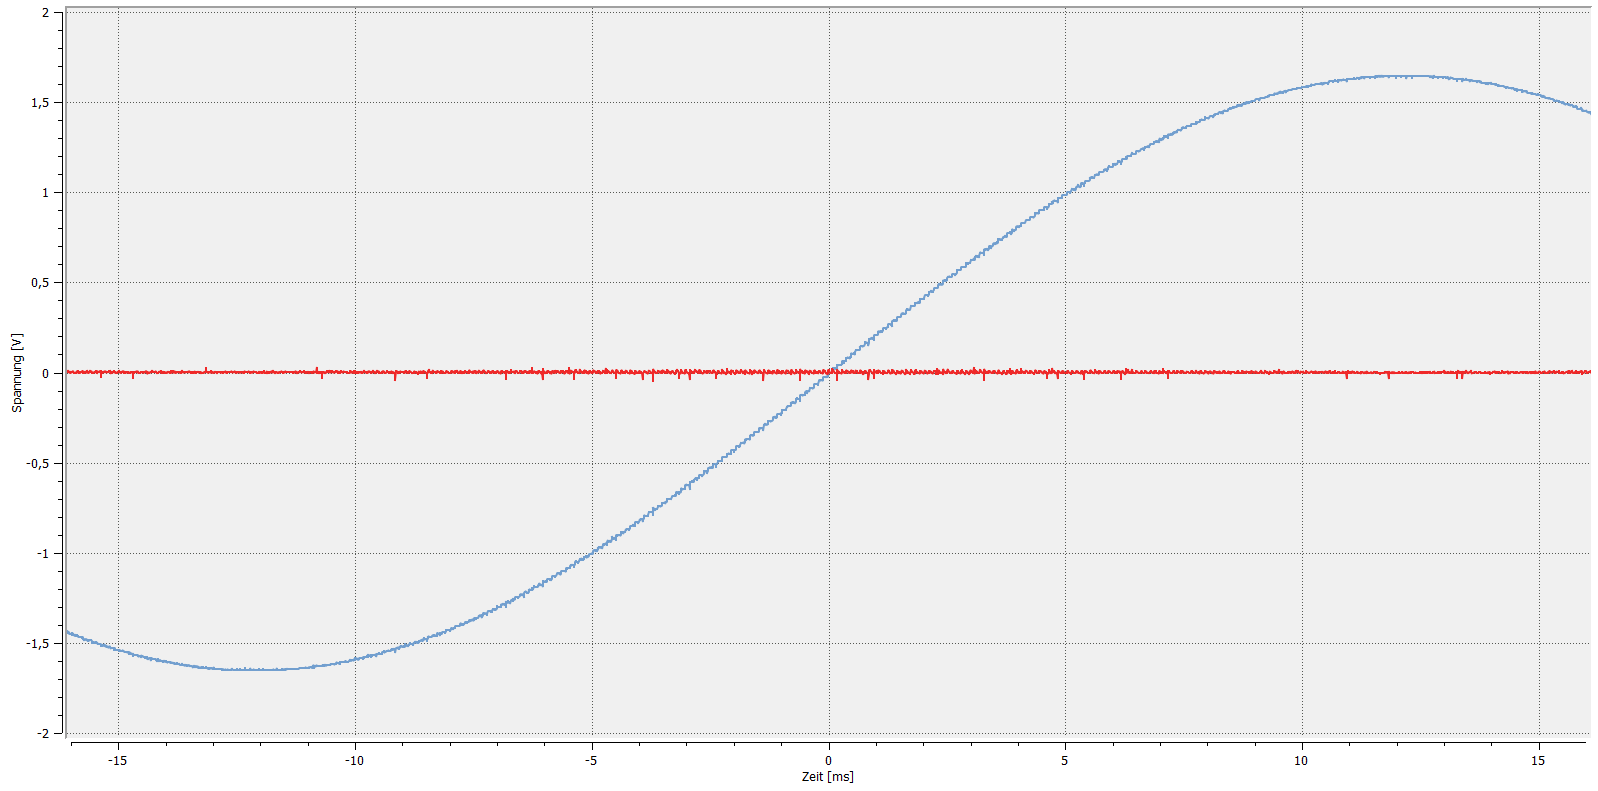
\includegraphics[width=0.49\textwidth]{pics/Hochpass 1,65V 20,6Hz Zeitbereich 32ms.PNG}}
	 \subfigure[Hochpass bei hohen Frequenzen]{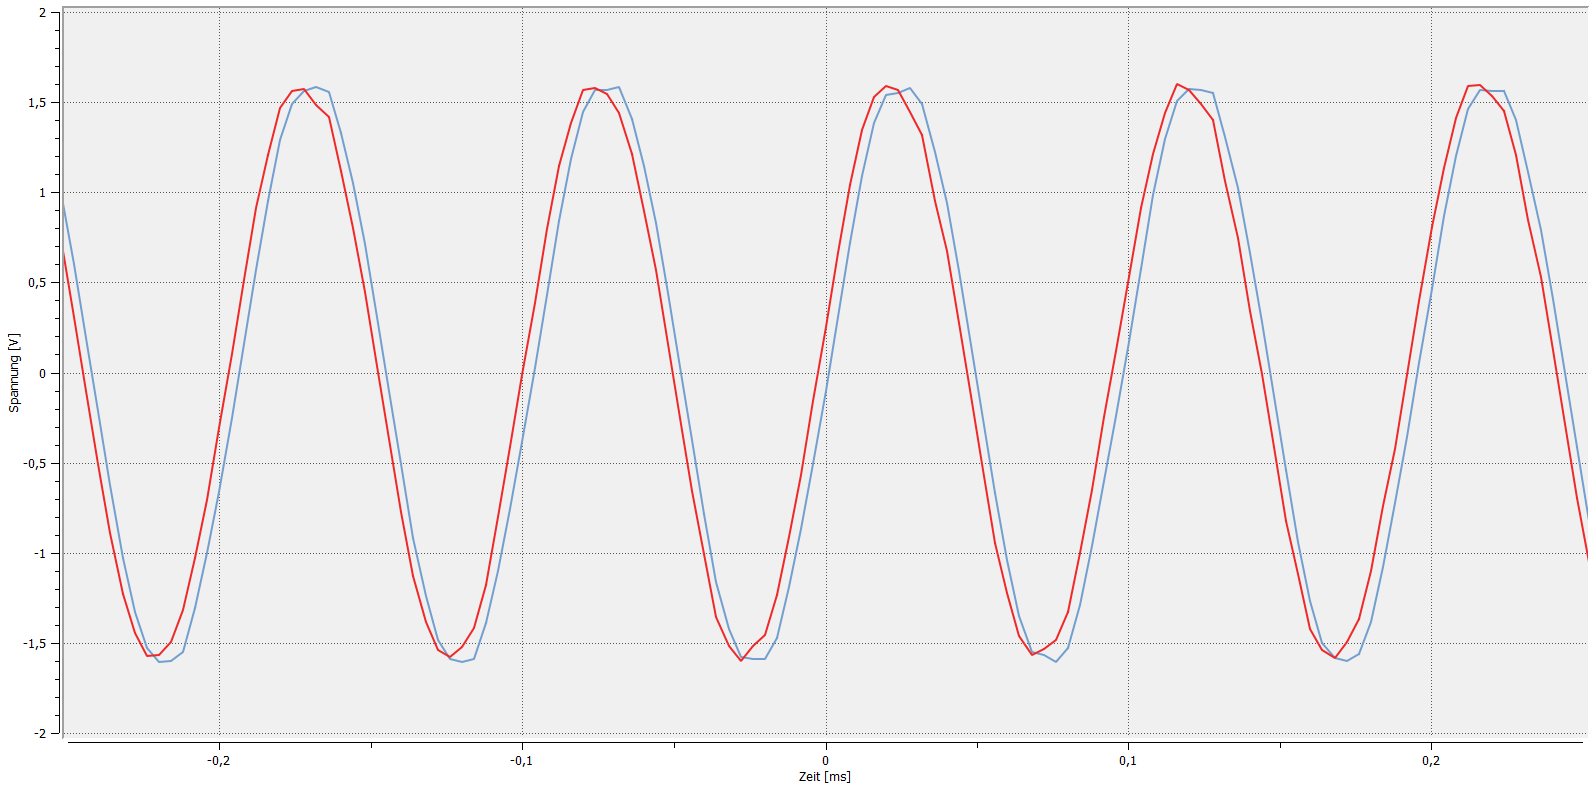
\includegraphics[width=0.49\textwidth]{pics/Hochpass 1,65V 10,3kHz Zeitbereich 0,5ms.PNG}}
  	\subfigure[Hochpass bei $\approx$1\si{\kilo\hertz}]{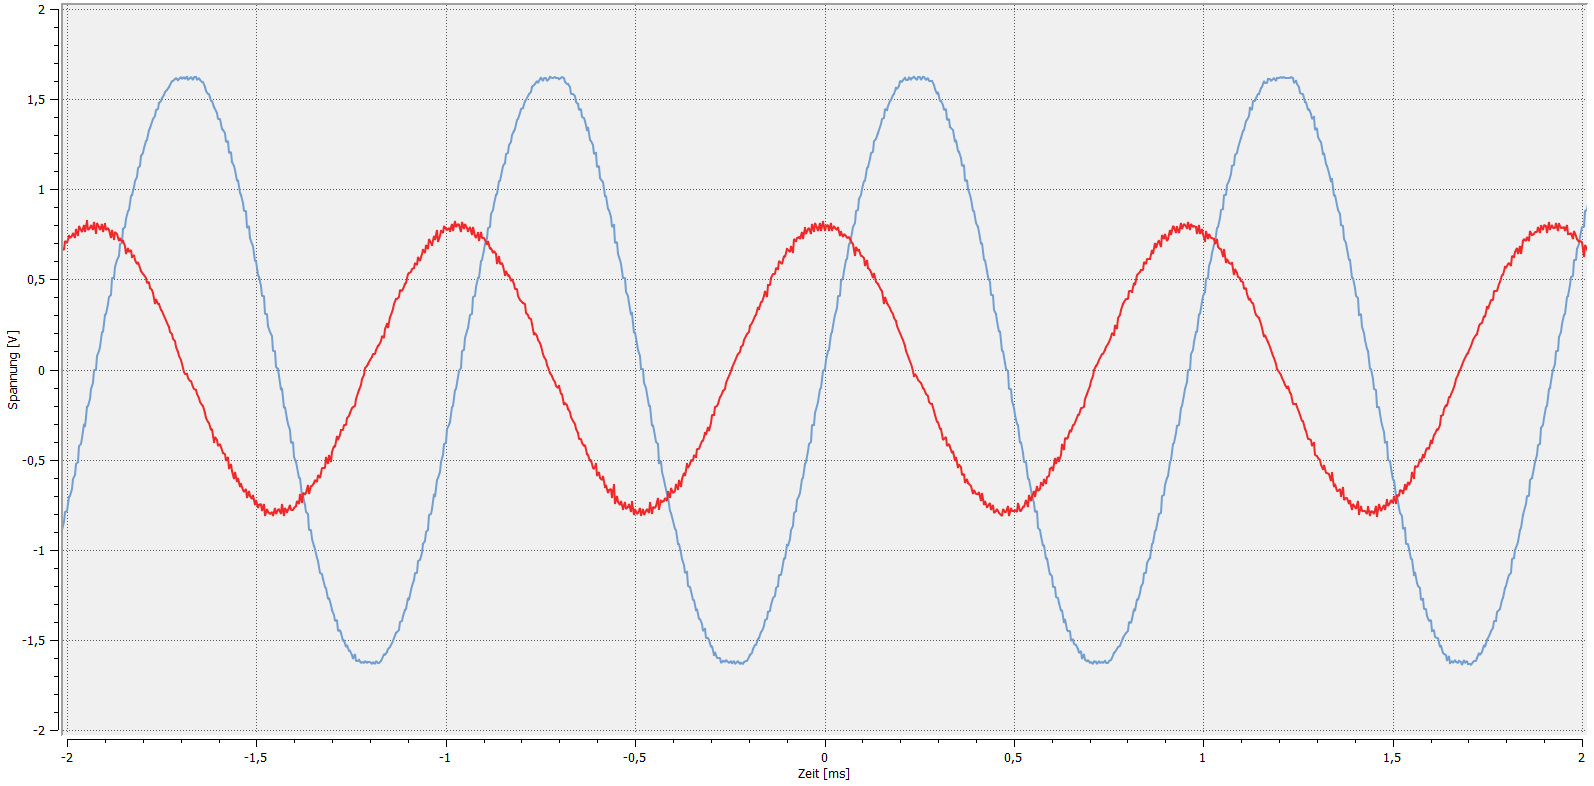
\includegraphics[width=0.49\textwidth]{pics/Hochpass 1,65V 1,04kHz Zeitbereich 4ms.PNG}}
  	\caption{Messungen des Hochpass mit Oszilloskop}  
  	\label{Hochpass Messung} 	
\end{figure}
In Bild (c) der Abbildung~\ref{Hochpass Messung} ist das Ausgangssignal, hier in Rot dargestellt, annähernd gleich dem Eingangssignal (blau). Gemessen wird hier bei einer Eingangsfrequenz von ~10\si{\kilo\hertz}. Bei niedrigen Frequenzen ist die Amplitude beim Ausgangssignal viel kleiner, also gedämpfter, als beim Eingangssignal. Dies ist in Bild (a) zu sehen. Bei einer Eingangsfrequenz von 20\si{hertz} ist die Amplitude des Ausgangssignals nahe Null. Der Hochpass erfüllt demnach seine Aufgabe des dämpfens niedriger Frequenzen. Bei der Grenzfrequenz beträgt die Amplitude des Ausgangssignals in etwa die Hälfte des Eingangssignals und ist um 90$^\circ$ phasenverschoben.\\
\\
Der Tiefpass funktioniert fungiert dem Hochpass gegenteilig. So lässt dieser niedrige Frequenzen nahezu eins zu eins durch. Zu sehen ist die in Bild (a) der Abbildung~\ref{Tiefpass Messung}, da hier die Linien des Eingangssignals (blau) und des Ausgangssignals (rot) in etwa die selbe Kurve beschreiben. Bei hohen Frequenzen (Bild (b)) ist das Ausgangssignal so verringert, dass kein Sinusverhalten zu erkennen ist. Beim Tiefpass wurden ebenfalls die Frequenzen 20\si{\hertz} und 10\si{\kilo\hertz} verwendet. Bei der Grenzfrequenz beträgt die Amplitude ebenfalls in etwa die Hälfte der Eingangsamplitude, die Phasenverschiebung beträgt -90$^\circ$.
\begin{figure}[H]
	\subfigure[Tiefpass bei tiefen Frequenzen]{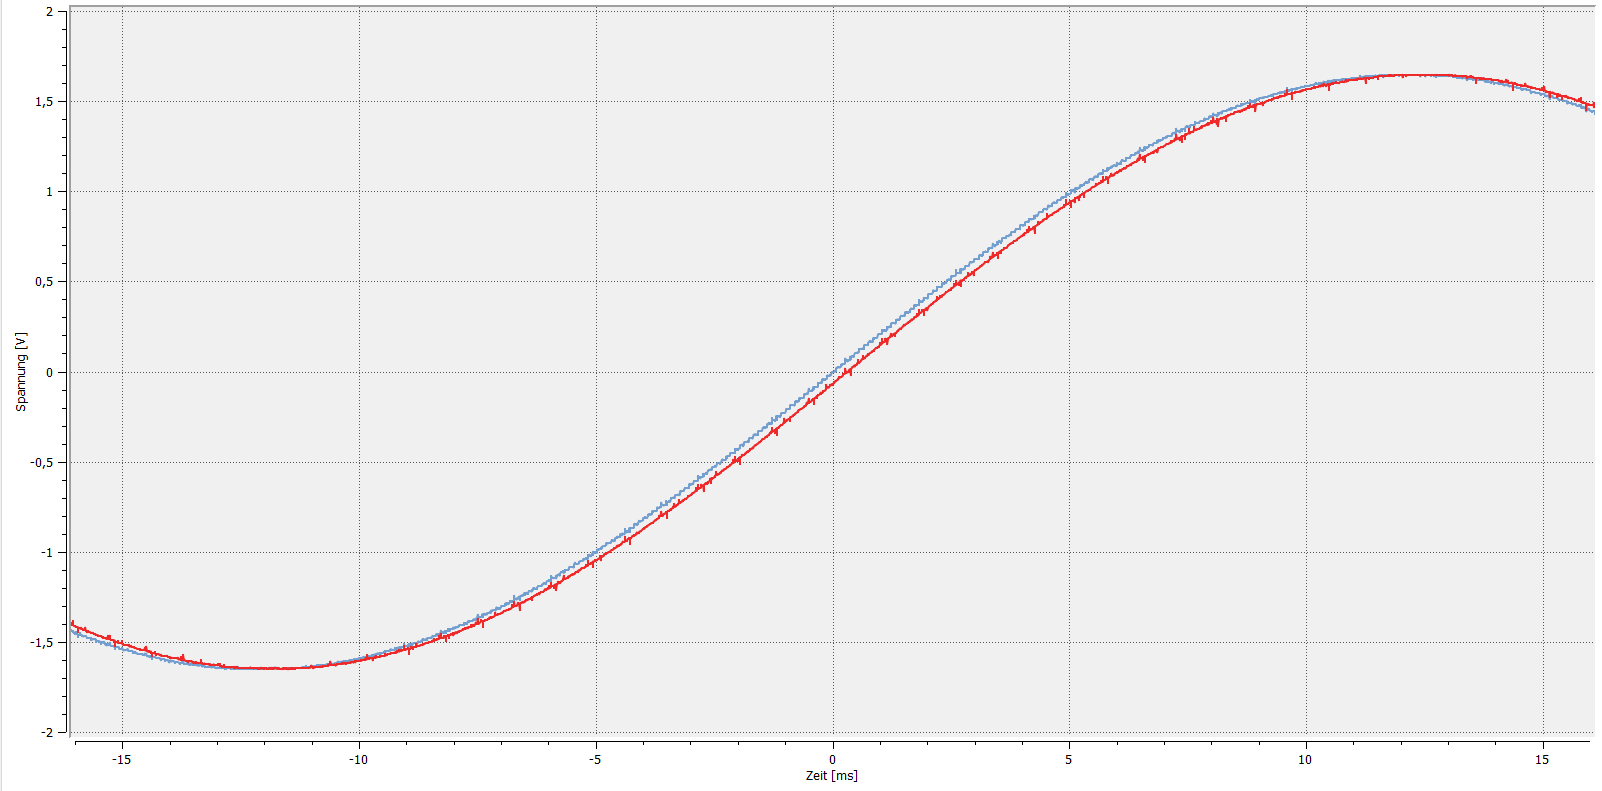
\includegraphics[width=0.49\textwidth]{pics/Tiefpass 1,65V 20,6Hz Zeitbereich 32ms.PNG}}
	 \subfigure[Tiefpass bei hohen Frequenzen]{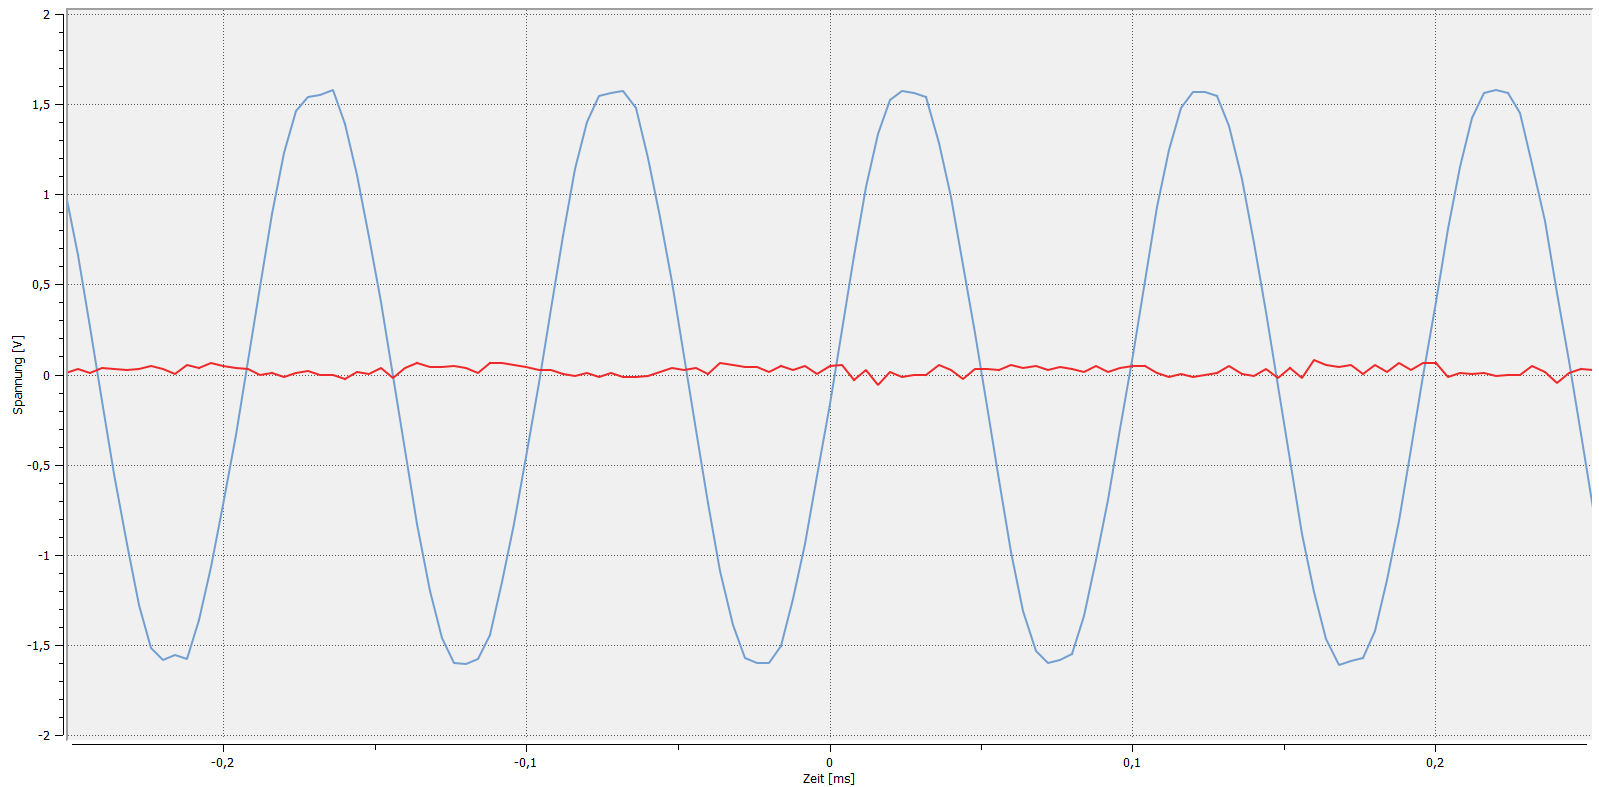
\includegraphics[width=0.49\textwidth]{pics/Tiefpass 1,65V 10,3kHz Zeitbereich 0,5ms.PNG}}
  	\subfigure[Tiefpass bei $\approx$1\si{\kilo\hertz}]{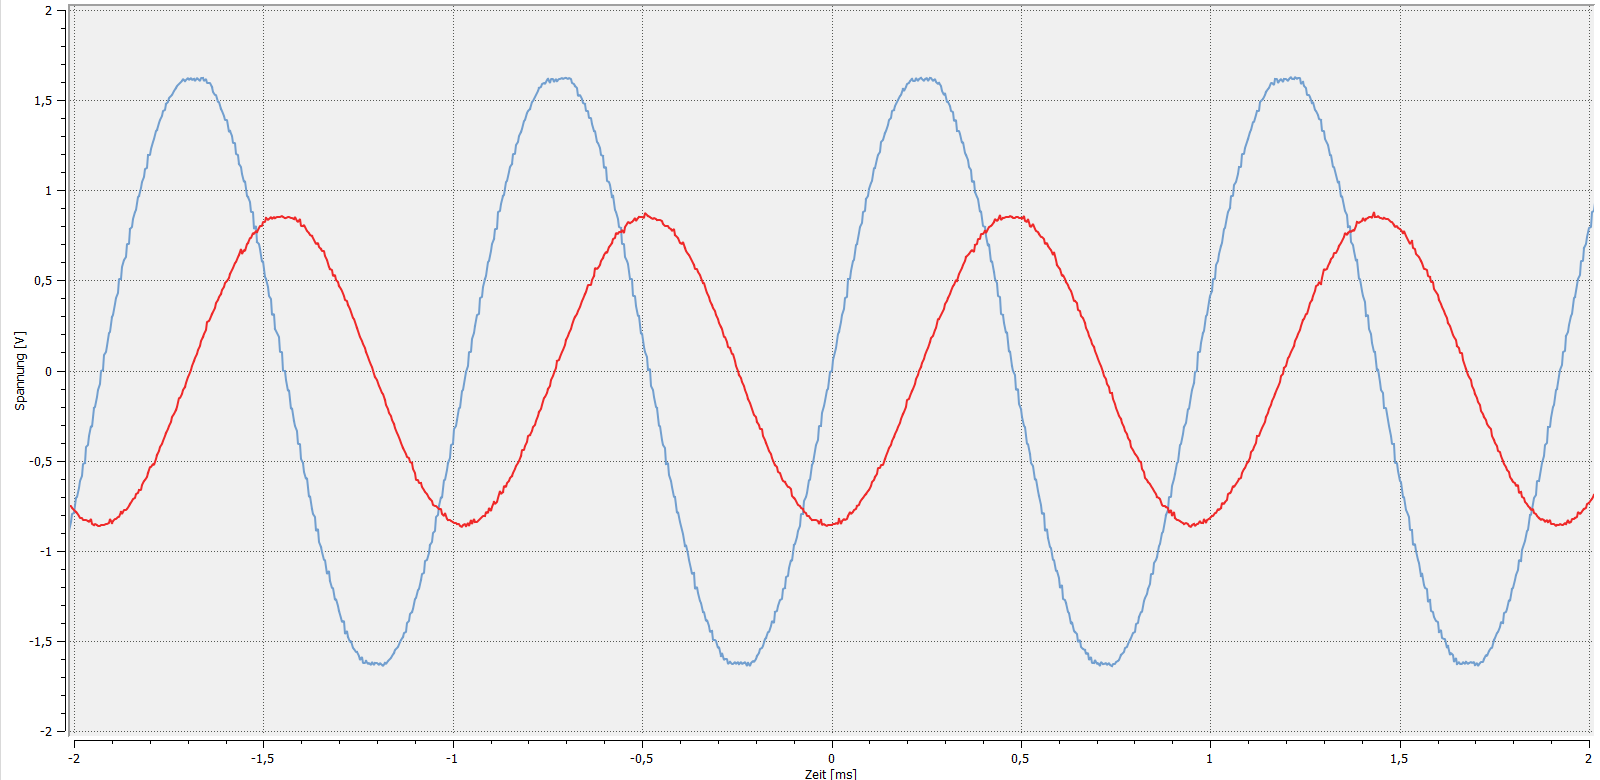
\includegraphics[width=0.49\textwidth]{pics/Tiefpass 1,65V 1,04kHz Zeitbereich 4ms.PNG}}
  	\caption{Messungen des Tiefpass mit Oszilloskop}  
  	\label{Tiefpass Messung} 	
\end{figure}
Die folgenden Diagramme stellen die simulierten Bode-Diagramme in LTSpice dar.
Hierbei zeigt die durchgezogenen Linie die Dämpfung in dB und die gestichelte Linie die Phase in Grad an.
\begin{figure}[H]
\subfigure[Bode-Diagramm des Hochpasses]{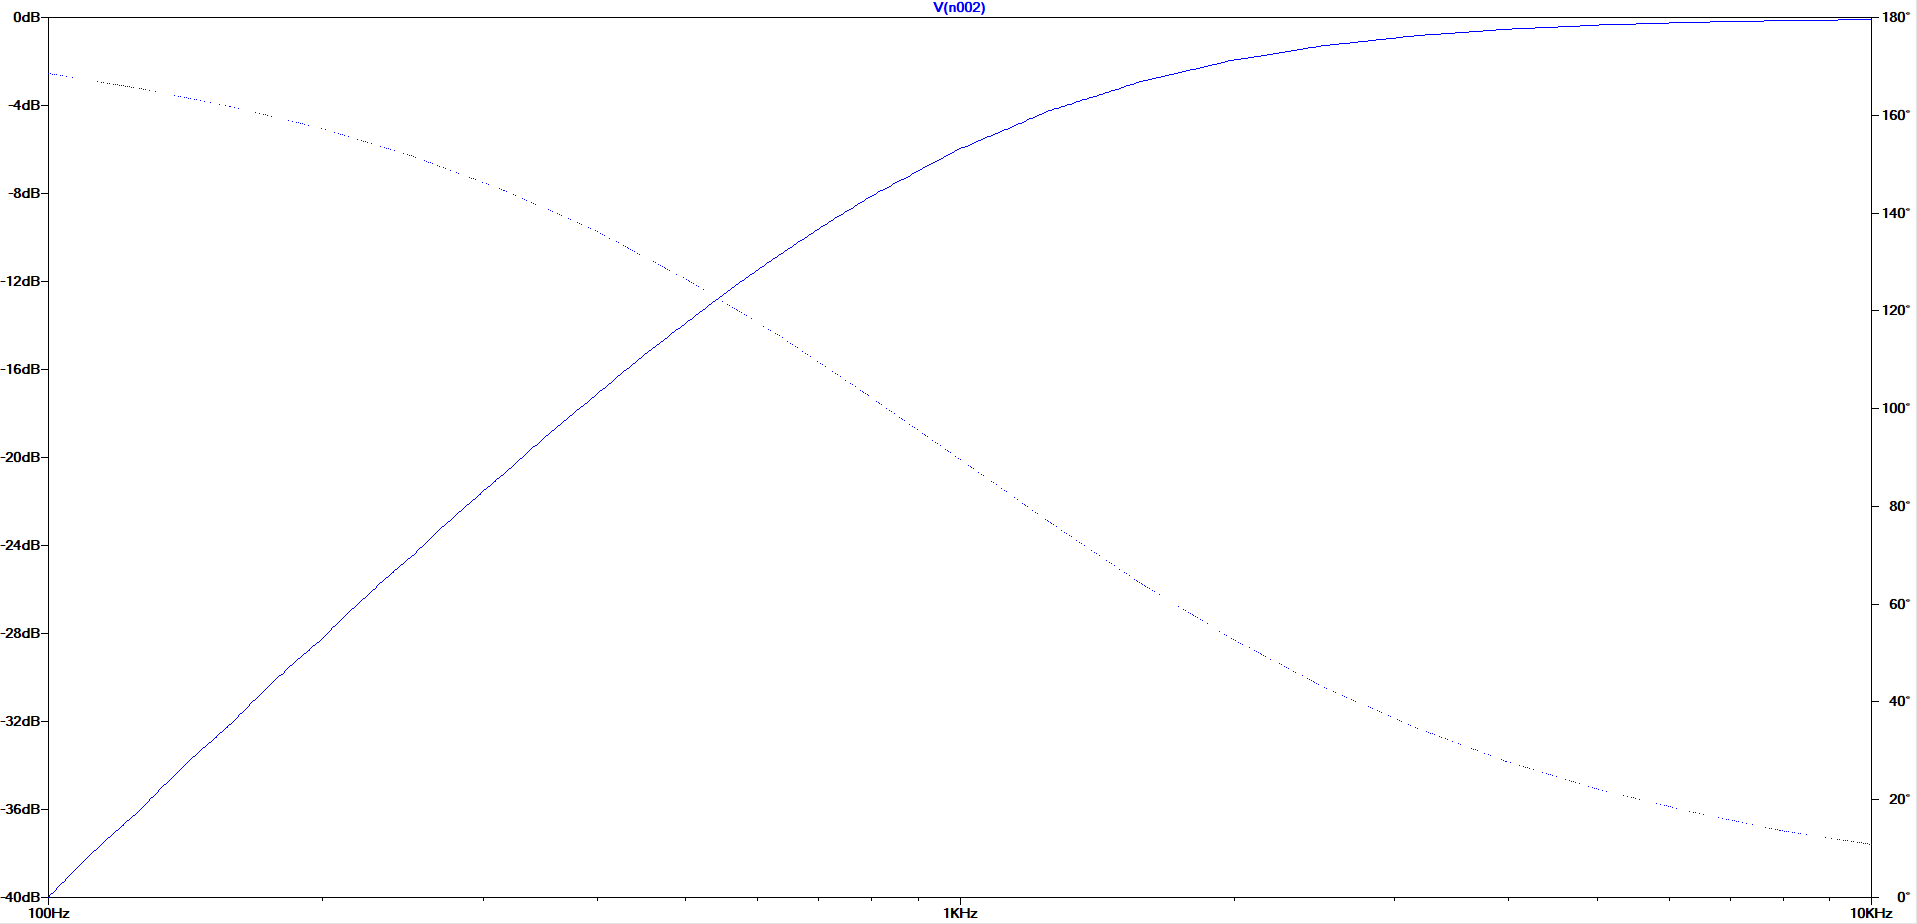
\includegraphics[width=0.49\textwidth]{pics/BodeSimHochpass.PNG}}
\subfigure[Bode-Diagramm des Tiefpasses]{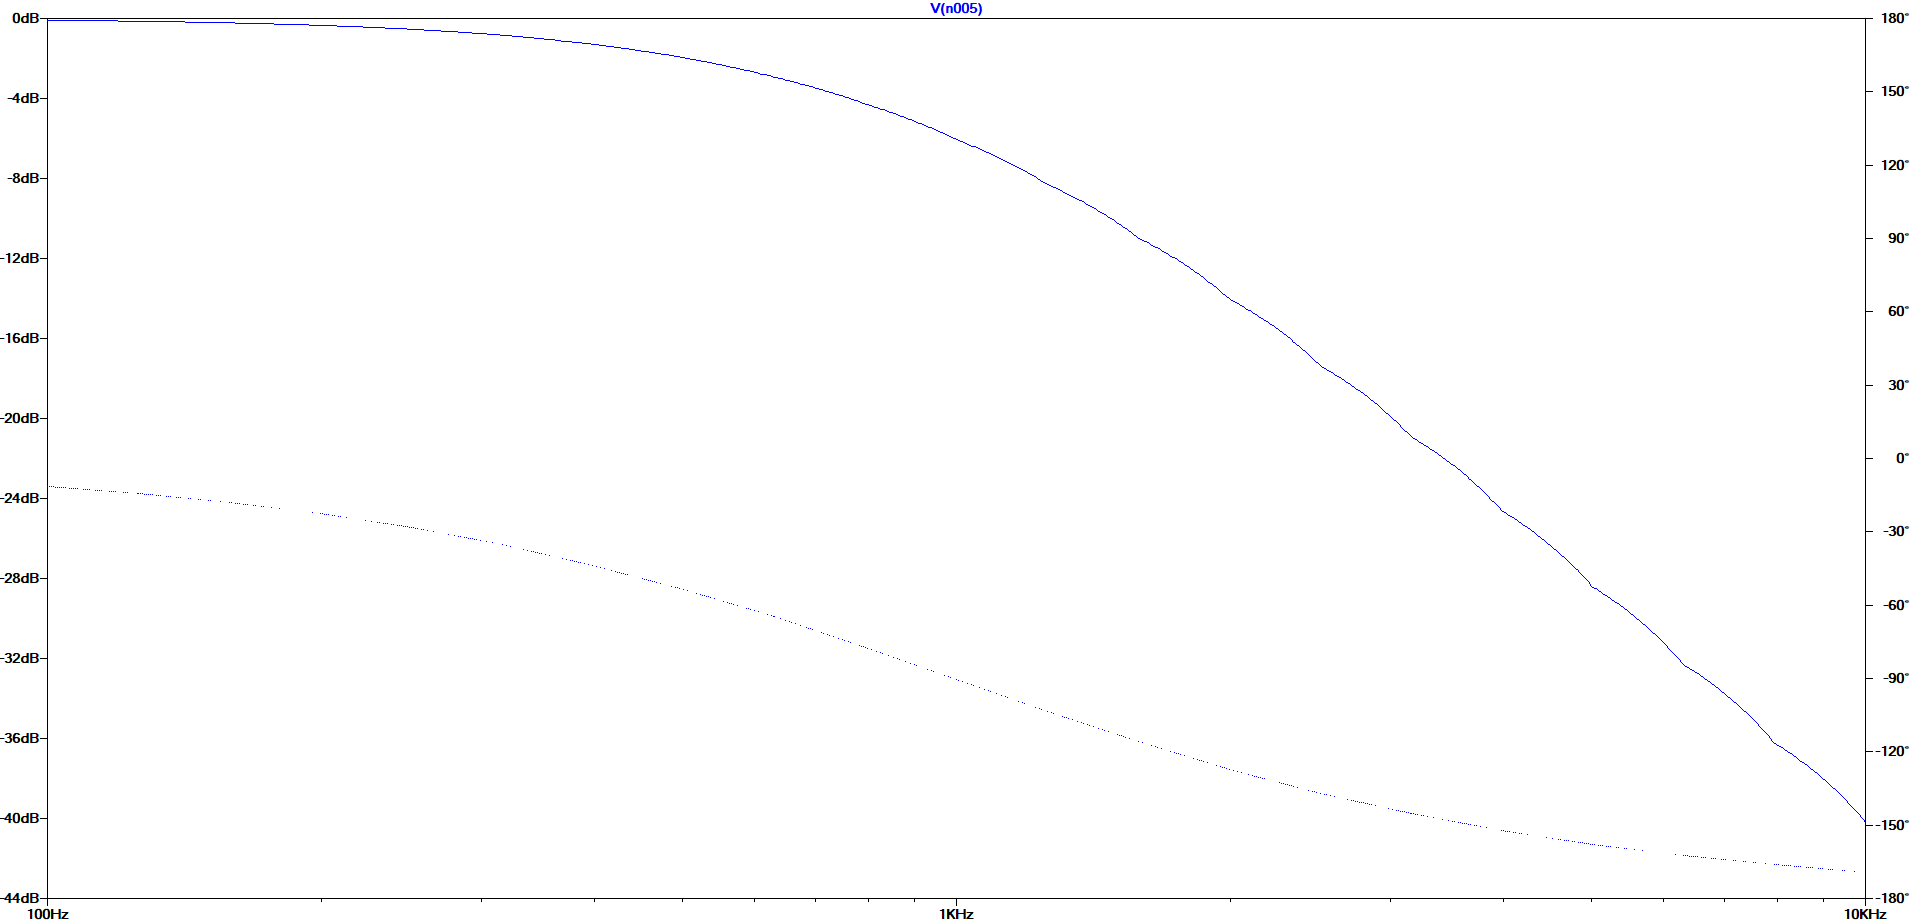
\includegraphics[width=0.49\textwidth]{pics/BodeSimTiefpass.PNG}}
\caption{Bode-Diagramme der Filter in LTSpice simuliert}
\label{Bode Spice}
\end{figure}
Durch messen der realen Schaltungen der Pässe auf dem Steckbrett erhält man folgende Bode-Diagramme. Die Messung wurde mittels der im Programm LENlab integrierten Frequenzanalyse durchgeführt.
\begin{figure}[H]
\subfigure[Bode-Diagramm des Hochpasses]{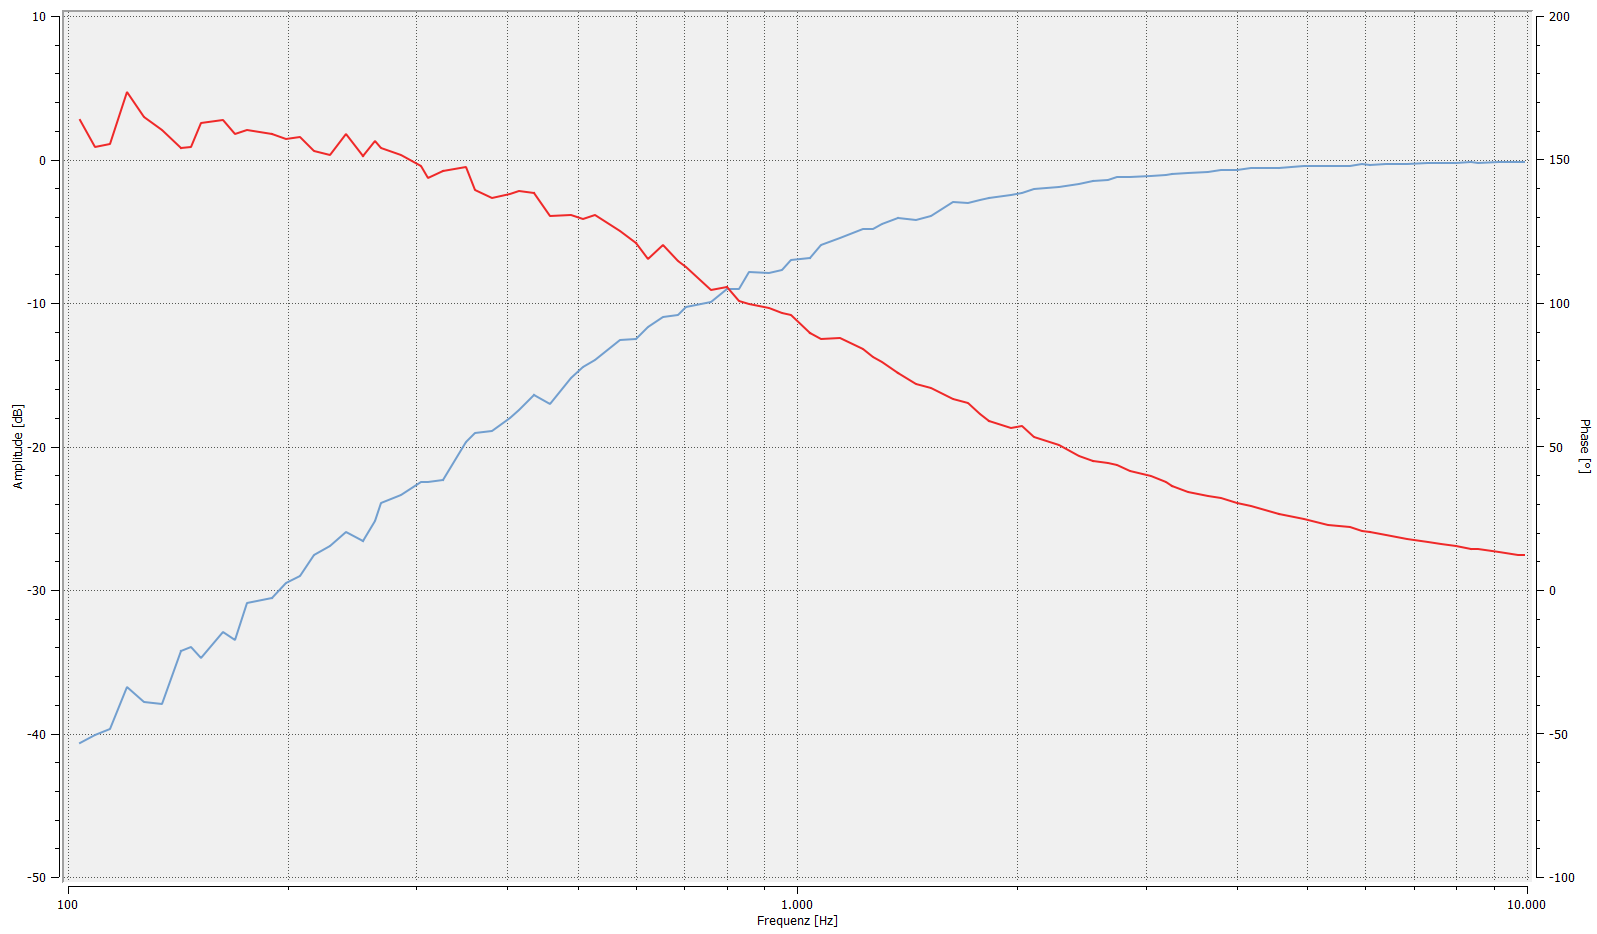
\includegraphics[width=0.49\textwidth]{pics/BodeHochpass.PNG}}
\subfigure[Bode-Diagramm des Tiefpasses]{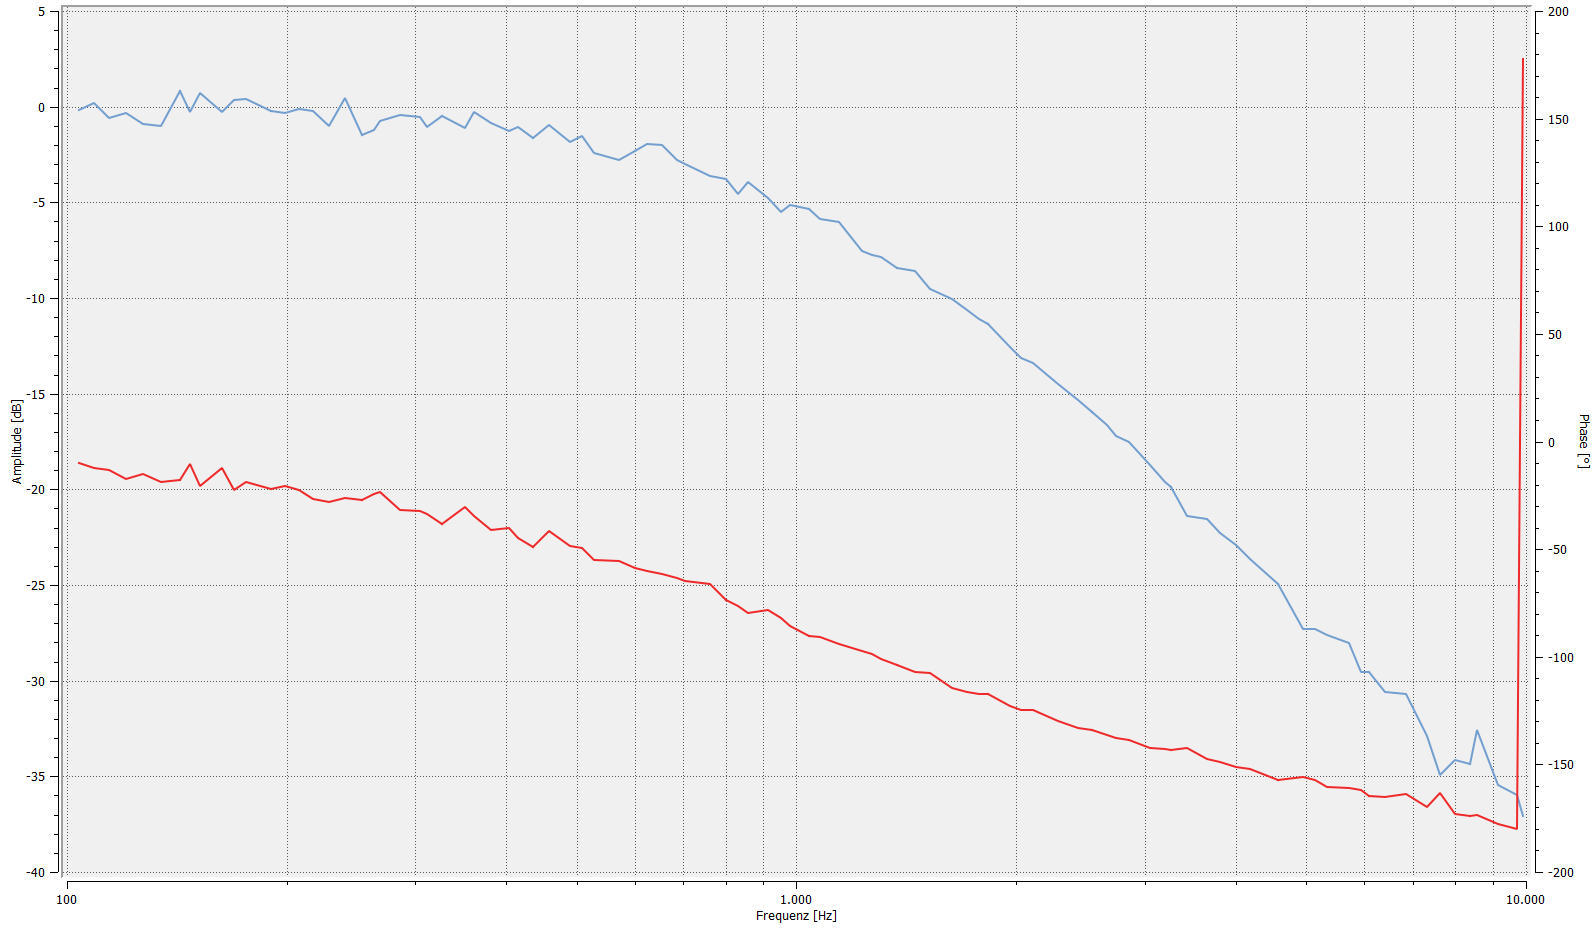
\includegraphics[width=0.49\textwidth]{pics/BodeTiefpass.PNG}}
\caption{Bode-Diagramme der Filter}
\label{Bode LENlab}
\end{figure}

\subsection{Diskussion}
Die Kurvenverläufe respektiven Bode-Diagramme stimmen mit den Simulationen maßgeblich überein. Ungenauigkeit gibt es zum Beispiel beim Sperrbereich des Tiefpass-Filters, dessen Kurve die -40\si{\dB} nicht gänzlich erreicht. Dies lässt sich jedoch auf kleiner Schwankungen oder Messungenauigkeiten zurückführen. Im Allgemeinen haben beide Filter eine Dämpfung im Sperrbereich von $\approx$-40\si{\dB}. Dieser Wert lässt sich sowohl aus der Simulation wie auch aus der Messung ziehen und bestätigt, dass es sich um Filter 2ter Ordnung handelt.\\
\\
Die größte Verstärkung ist bei den Simulierten Diagrammen bei 0\si{\dB}. Somit haben wir den gewollten Verstärkungsfaktor von 1 im Durchlassbereich. Dies zeigt sich auch in den Diagrammen der realen Messungen, wobei sich die Kurve des Hochpasses glatt der Null nähert und die Kurve des Tiefpasses bei niedrigen Frequenzen sogar kurzzeitig über die 0dB Grenze springt. Dieses Verhalten entsteht durch Messungenauigkeiten bei niedrigen Frequenzen.\\
\\
Diese zeigen sich auch bei der gemessenen Kurve der Phasenverschiebung des Hochpasses. Insgesamt zeigen die gemessenen Diagramme die erwartet Änderung der Phasenverschiebung von $\pm 180^\circ$ besser als die Simulation. Dies stellen die Bilder aus Abbildung~\ref{Hochpass Messung} und \ref{Tiefpass Messung} recht gut dar. Zwischen 100\si{\hertz} und der Grenzfrequenz ändert sich die Phase um 90$^\circ$ und von der Grenzfrequenz bis 10\si{\kilo\hertz} nochmals um 90$^\circ$. So liegen die jeweiligen Kurven von Abbildung~\ref{Hochpass Messung} (b) und die von Abbildung~\ref{Tiefpass Messung} (a) aufeinander, d.h. Ausgangsspannung und Eingangsspannung sind Phasengleich. Hierbei gibt es im Graphen des Tiefpassfilters eine Besonderheit. Der Sprung kurz vor der Frequenz 10\si{\kilo\hertz} kommt daher, dass LENlab das Ende der zyklischen Skala erreicht und bei $\pm 180^\circ$ entweder 360$^\circ$ abzieht oder hinzufügt.\\
\\
Bei der Simulation liegt die Grenzfrequenz genau bei den vorhergesagten -6dB (Filter 2. Ordnung). Bestimmt man allerdings im Bode-Diagramm des Tiefpass-Filters die Frequenz bei -6dB, so liegt diese leicht über 1\si{\kilo\hertz}. Dies liegt and Schwankungen in der Messdurchführung. Würde man die Kurve glätten würde man die vorhergesagte Grenzfrequenz treffen.\\
\\
Abschließend lässt sich festhalten, dass die Eigenschaften der Filter den Anforderungen der Aufgabenstellung gerecht werden. Der Tiefpass die tiefen Frequenzen durch und dämpft die hohen. Analog dämpft der Hochpass die tiefen Frequenzen und lässt die hohen durch. Beide Filter verstärken im Durchlassbereich um den Faktor 1 und die Grenzfrequenz liegt bei 1\si{\kilo\hertz}. Dies zeigt sowohl die LTSpice Simulation der Schaltung wie auch die Messungen in mit Steckbrett und LENlab. Somit können beide Filter für die nächste Problemstelle, das zusammenführen der Ausgangssignale mittels einer Addiererschaltung, verwendet werden. 


\section{Aufgabe 2}
Erklärsatz

\subsection{Methoden}
bla bla Methoden

\subsection{Ergebnisse}
bla bla Ergebnisse

\subsection{Diskussion}
bla bla Diskussion






\clearpage % neue Seite beginnen
\begin{thebibliography}{99}

\bibitem{radio} \url{https://www.bundesnetzagentur.de/SharedDocs/Downloads/DE/Sachgebiete/Telekommunikation/Unternehmen_Institutionen/Frequenzen/20191202_Frequenzplan.pdf;jsessionid=9ADB9CCA7A684BFDF08E57A768012FE1?__blob=publicationFile&v=2} Abgerufen: 22.01.2020, (Seite 190,Eintrag 203003)

\bibitem{Wiki Equalizer} \url{https://de.wikipedia.org/wiki/Equalizer} Abgerufen: 25.01.2020, 10:56 Uhr
\bibitem{IBK} \url{https://www.elektronik-kompendium.de/sites/grd/1006231.htm}
Abgerufen: 28.01.2w
\bibitem{IBS} \url{https://www.elektronik-kompendium.de/sites/grd/1006241.htm} Abgerufen: 28.01.2020
\bibitem{skript} Vorlesungsskript zur Vorlesung Lineare Elektrische Netze, Prof. Dr. rer. nat. Olaf Dössel, Institut für biomedizinische Technik
\bibitem{DSV} Digitale Signalverarbeitung : Filterung und Spektralanalyse mit MATLAB-Übungen / Karl-Dirk Kammeyer, Kristian Kroschel Jahr:2018, ISBN: 3-658-20134-7s



\bibitem{Hoerbereichdiagramm} Buch: Hörbereiche nach: Schmidt, Lang. Physiologie des Menschen. Ausgabe: Springer(2007)






%\bibitem{cite} \url{http://www.starkerstart.uni-frankfurt.de/43759138/FB09-Musikwissenschaften-Richtiges-Zitieren.pdf}, Abrufdatum: 30.11.2016.
%\bibitem{atmel} Atmel Corporation. 32-bit ATMEL AVR Microcontroller AT32UC3B0256. \url{http://www.atmel.com/devices/at32uc3b0256.aspx}, Abrufdatum: 15. Oktober 2013.
%\bibitem{bronstein} I. N. Bron\v{s}tejn, K. A. Semendjajew, G. Musiol und H. Mühlig (Hrsg.). {\itshape Taschenbuch der Mathematik}. Verlag Harri Deutsch, Frankfurt am Main, 8. Auflage, 2012.
%\bibitem{kalman} R. E. Kalman. A New Approach to Linear Filtering and Prediction Problems. In: {\itshape Transactions of the ASME--Journal of Basic Engineering}, Bd. 82 (D), S. 35--45, 1960.
\end{thebibliography}


\end{document}

